\documentclass[12pt,fontset=fandol]{ctexart}
\usepackage[a4paper,margin=1in]{geometry}
\usepackage{booktabs}
\usepackage{graphicx}
\usepackage{float}
\usepackage{hyperref}
\usepackage{longtable}
\usepackage{array}
\usepackage{xcolor}
\usepackage{listings}

\title{TCGA-LIHC 肿瘤/正常样本分类实验报告}
\author{学院：元培学院 \quad 姓名：高禹宸}
\date{\today}

\lstset{
  basicstyle=\ttfamily\small,
  breaklines=true,
  frame=single,
  columns=fullflexible,
  keepspaces=true,
  showstringspaces=false
}


\begin{document}
\maketitle

\section{实验目的}
本实验使用 TCGA GDC Liver Cancer 表达量数据，对肿瘤样本与正常样本进行二分类分析。实验目标包括：
\begin{itemize}
  \item 掌握 TCGA 表达量矩阵的基本读取与样本类型识别方法；
  \item 掌握基于训练集进行差异基因筛选和特征选择的基本流程；
  \item 使用合适的机器学习方法完成肿瘤/正常样本分类；
  \item 通过可视化和评价指标理解模型结果及其局限性。
\end{itemize}

\section{背景介绍}
肝细胞癌是一种比较常见的恶性肿瘤。肿瘤样本和正常样本在基因表达水平上通常会有比较明显的差异，因此可以尝试用表达谱数据把它们区分开。本实验使用 TCGA-LIHC 的表达量矩阵，并根据 TCGA barcode 里的样本类型编码区分肿瘤样本和正常样本。其中：\texttt{01} 表示原发肿瘤样本，\texttt{11} 表示正常组织样本，\texttt{02} 为其他类型样本，这部分不纳入本次分析。

本次实验也是对于机器学习方法的一次实践与了解。此方法将样本的特征和它对应的正确类别交给模型，让模型去学习两者之间的关系，进而做出我们所需要的预测。在这个实验里，输入特征是很多个基因的表达量，标签则是样本为肿瘤还是正常。整个机器学习流程为：整理数据，选择合适的方法训练模型，测试模型预测能力。

本实验利用决策树来做分类。决策树根据特征一步一步地做判断，把样本分到不同类别里。它的优点是结构清楚，容易解释，也方便看出哪些基因对分类更重要；单如果出现树长得太复杂的情况，可能会把训练数据记得太死，影响泛化能力。

\section{实验方法}
\subsection{数据来源与样本筛选}
本次实验使用文件 \texttt{TCGA-LIHC.star\_counts (2).tsv.gz}。数据共有 60660 个基因条目和 424 个样本列。根据 TCGA barcode 第 14--15 位的样本类型编码进行分组：
\begin{itemize}
  \item \texttt{01}：Primary Tumor，记为 Tumor
  \item \texttt{11}：Solid Tissue Normal，记为 Normal
  \item \texttt{02}：其他类型，本实验不纳入建模
\end{itemize}

对应的 R 代码如下：
\begin{lstlisting}[language=R]
raw_df <- read.delim(gzfile("TCGA-LIHC.star_counts (2).tsv.gz"), check.names = FALSE)
ensembl_id <- sub("\\..*$", "", raw_df[[1]])
sample_ids <- colnames(raw_df)[-1]
sample_type_code <- substr(sample_ids, 14, 15)
keep_idx <- sample_type_code %in% c("01", "11")
labels <- factor(
  ifelse(sample_type_code[keep_idx] == "01", "Tumor", "Normal"),
  levels = c("Normal", "Tumor")
)
\end{lstlisting}

\begin{table}[H]
\centering
\caption{原始样本类型统计}
\begin{tabular}{ccc}
\toprule
样本类型编码 & 分组 & 数量 \\
\midrule
01 & Tumor & 371 \\
11 & Normal & 50 \\
02 & Other & 3 \\
\bottomrule
\end{tabular}
\end{table}

最终用于分类的样本共有 421 个，其中 Tumor 371 个，Normal 50 个。

\subsection{数据预处理}
预处理步骤如下：
\begin{itemize}
  \item 读取表达矩阵，提取 Ensembl ID，并去除版本号后缀；
  \item 仅保留样本类型编码为 \texttt{01} 和 \texttt{11} 的样本；
  \item 以样本为行、基因为列构建机器学习输入矩阵；
  \item 使用 \texttt{bitr()} 和 \texttt{org.Hs.eg.db} 将 Ensembl ID 尽可能转换为基因 Symbol，用于结果展示和图像标注。
\end{itemize}

对应的 R 代码如下：
\begin{lstlisting}[language=R]
expr_mat <- as.matrix(raw_df[, -1, drop = FALSE])[, keep_idx, drop = FALSE]
rownames(expr_mat) <- ensembl_id

gene_map <- bitr(
  unique(ensembl_id),
  fromType = "ENSEMBL",
  toType = "SYMBOL",
  OrgDb = org.Hs.eg.db,
  drop = FALSE
)
colnames(gene_map)[colnames(gene_map) == "ENSEMBL"] <- "ENSEMBL_clean"
\end{lstlisting}

\subsection{数据分割}
采用分层抽样的方式进行 7:3 训练集/测试集划分，以保证训练集和测试集中都保留肿瘤与正常样本。

对应的 R 代码如下：
\begin{lstlisting}[language=R]
set.seed(20260403)
train_idx <- unlist(
  tapply(seq_along(labels), labels, function(i) sample(i, ceiling(length(i) * 0.7)))
)
test_idx <- setdiff(seq_along(labels), train_idx)

train_expr <- expr_mat[, train_idx, drop = FALSE]
test_expr <- expr_mat[, test_idx, drop = FALSE]
train_labels <- labels[train_idx]
test_labels <- labels[test_idx]
\end{lstlisting}

\begin{table}[H]
\centering
\caption{训练集与测试集样本统计}
\begin{tabular}{cccc}
\toprule
数据集 & Tumor & Normal & 合计 \\
\midrule
Training & 260 & 35 & 295 \\
Testing & 111 & 15 & 126 \\
\bottomrule
\end{tabular}
\end{table}

\subsection{特征选择}
为避免信息泄漏，先划分训练集与测试集，再仅在训练集上进行差异表达分析。具体做法如下：
\begin{itemize}
  \item 对每个基因在 Tumor 与 Normal 之间做 Welch t 检验；
  \item 使用 Benjamini-Hochberg 方法对 p 值进行多重检验校正；
  \item 按校正后 p 值从小到大排序，并结合 $|LogFC|$ 进行筛选；
  \item 取前 50 个差异表达最显著的基因作为模型输入特征。
\end{itemize}

对应的 R 代码如下：
\begin{lstlisting}[language=R]
tumor_mean <- rowMeans(train_expr[, train_labels == "Tumor", drop = FALSE])
normal_mean <- rowMeans(train_expr[, train_labels == "Normal", drop = FALSE])
log_fc <- tumor_mean - normal_mean
p_value <- apply(train_expr, 1, function(v) {
  t.test(v[train_labels == "Tumor"], v[train_labels == "Normal"])$p.value
})
padj <- p.adjust(p_value, method = "BH")

de_table <- data.table(
  Gene = rownames(train_expr),
  LogFC = log_fc,
  PValue = p_value,
  Padj = padj
)
setorder(de_table, Padj, -abs(LogFC))
top50_genes <- de_table$Gene[1:50]
\end{lstlisting}

\subsection{模型训练}
本实验的建模流程比较直接：先把样本按类别分开抽样，再只在训练集里筛选 Top50 差异表达基因，最后用这些基因训练二分类决策树模型。

模型训练参数设置为：
\begin{itemize}
  \item \texttt{method = "class"}，用于二分类；
  \item \texttt{cp = 0.001}；
  \item \texttt{maxdepth = 5}；
  \item \texttt{minbucket = 4}；
  \item 使用平衡先验概率 \texttt{prior = c(0.5, 0.5)}，减轻类别不平衡影响。
\end{itemize}

对应的 R 代码如下：
\begin{lstlisting}[language=R]
train_df <- data.frame(Class = train_labels, t(train_expr[top50_genes, , drop = FALSE]))
test_df <- data.frame(Class = test_labels, t(test_expr[top50_genes, , drop = FALSE]))

tree_model <- rpart(
  Class ~ .,
  data = train_df,
  method = "class",
  parms = list(prior = c(0.5, 0.5)),
  control = rpart.control(cp = 0.001, maxdepth = 5, minbucket = 4)
)
\end{lstlisting}

\section{实验结果}
\subsection{差异表达基因结果}
训练集中前 10 个差异表达基因如下表所示。这些基因在 Tumor 与 Normal 之间具有较明显的表达差异，可作为后续分类模型的重要输入特征。

\begin{table}[H]
\centering
\caption{训练集中前 10 个差异表达基因}
\begin{tabular}{lrrr}
\toprule
Gene Symbol & LogFC & PValue & Padj \\
\midrule
GDF2 & -8.2757 & 4.14E-86 & 2.31E-81 \\
SFTA1P & 3.2325 & 1.33E-78 & 3.73E-74 \\
CXCL14 & -6.2229 & 3.87E-77 & 7.21E-73 \\
SFRP5 & -6.2469 & 6.00E-73 & 8.37E-69 \\
CHST4 & -5.6493 & 8.43E-69 & 9.39E-65 \\
COLEC10 & -5.4778 & 1.01E-68 & 9.39E-65 \\
SLC5A1 & -5.0420 & 2.87E-65 & 2.29E-61 \\
BMP10 & -6.8837 & 1.39E-63 & 9.69E-60 \\
SLC25A47 & -4.9568 & 2.63E-61 & 1.63E-57 \\
ENSG00000243694 & -4.6418 & 7.04E-60 & 3.93E-56 \\
\bottomrule
\end{tabular}
\end{table}

\begin{figure}[H]
\centering
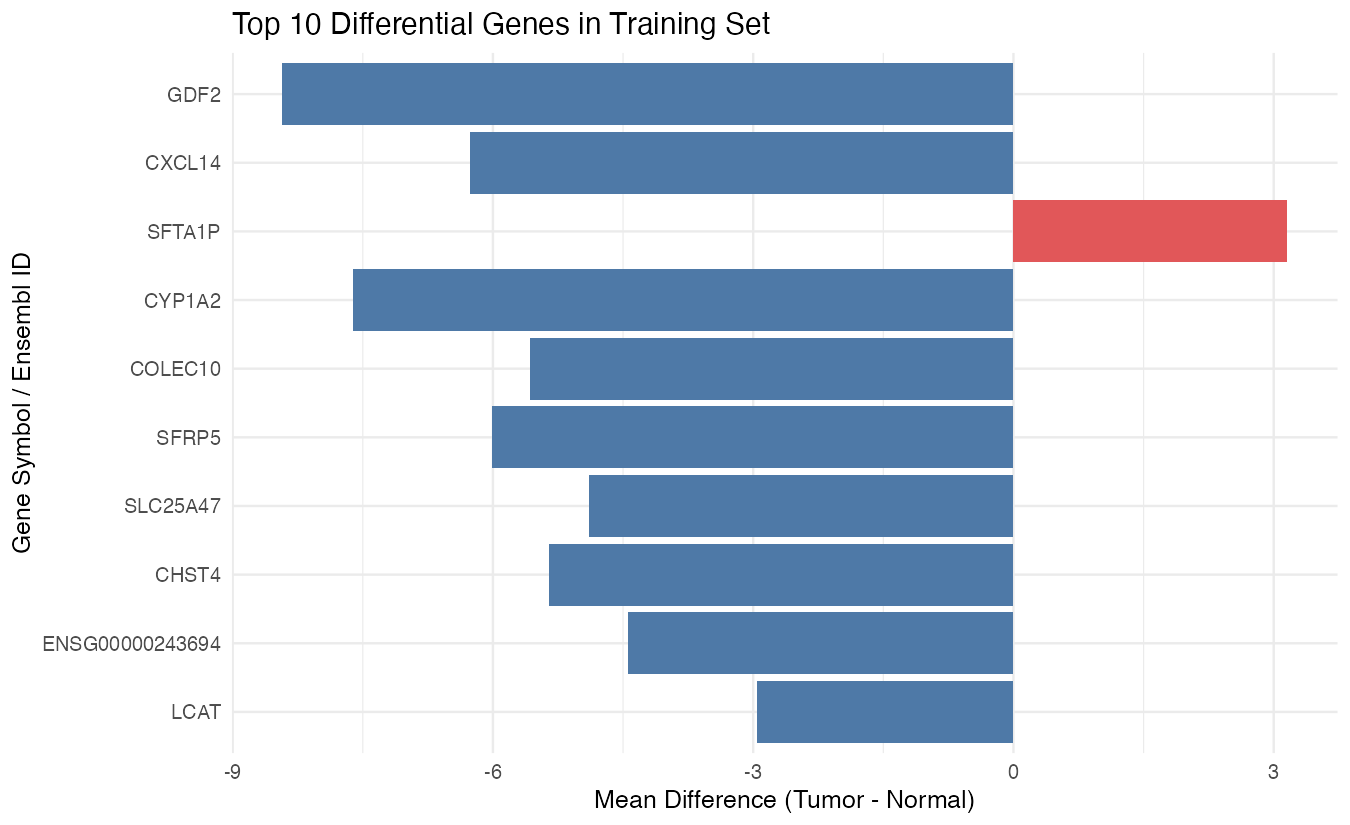
\includegraphics[width=0.78\textwidth]{tcga_hw_outputs/figures/top10_differential_genes.png}
\caption{前 10 个差异表达基因可视化}
\end{figure}

从图中可以看出，这些基因在 Tumor 与 Normal 间的表达差异方向并不完全一致，其中部分基因在正常样本中表达更高，部分基因在肿瘤样本中表达更高，这说明分类信息并不是由单一方向的表达变化决定，而是由多基因组合共同决定。

\subsection{样本分布的 PCA 结果}
\begin{figure}[H]
\centering
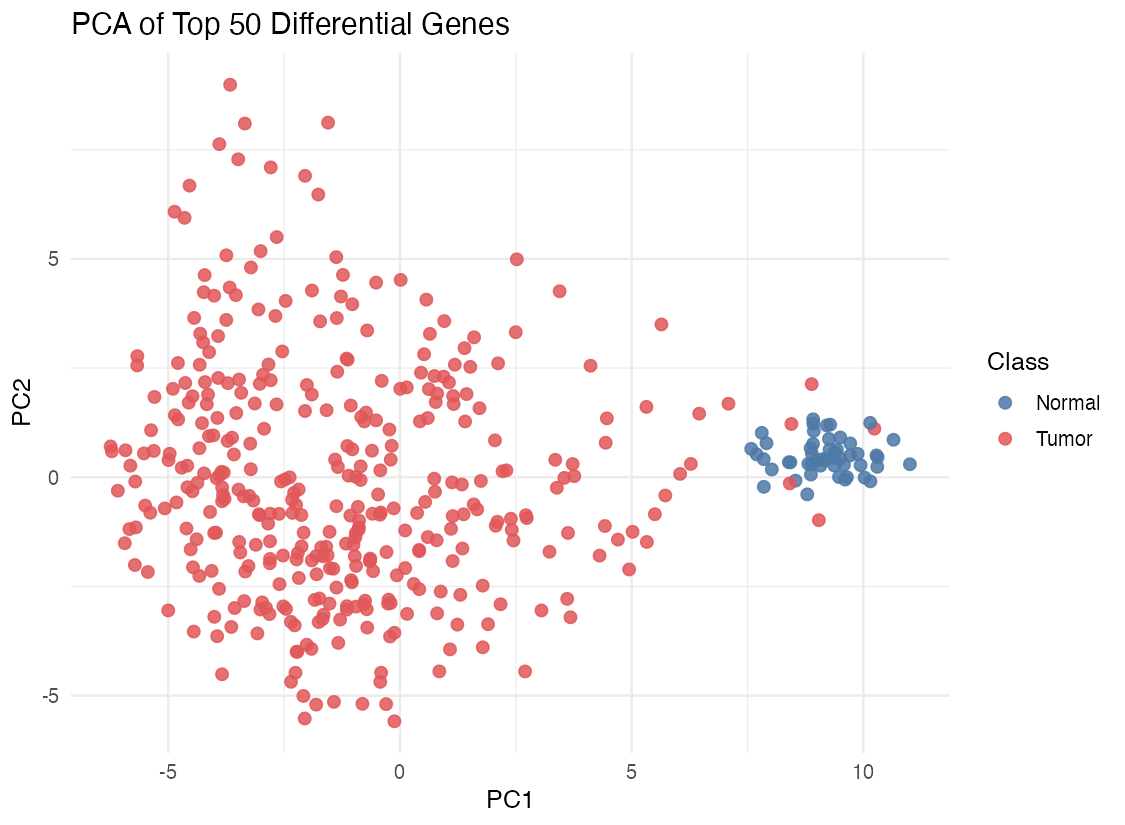
\includegraphics[width=0.72\textwidth]{tcga_hw_outputs/figures/pca_top50.png}
\caption{Top50 差异基因的 PCA 可视化}
\end{figure}

PCA 结果显示，肿瘤样本与正常样本在前两个主成分空间中已经出现较明显分离，说明筛选出的差异基因具有较好的判别能力。

\subsection{决策树结构与重要变量}
\begin{figure}[H]
\centering
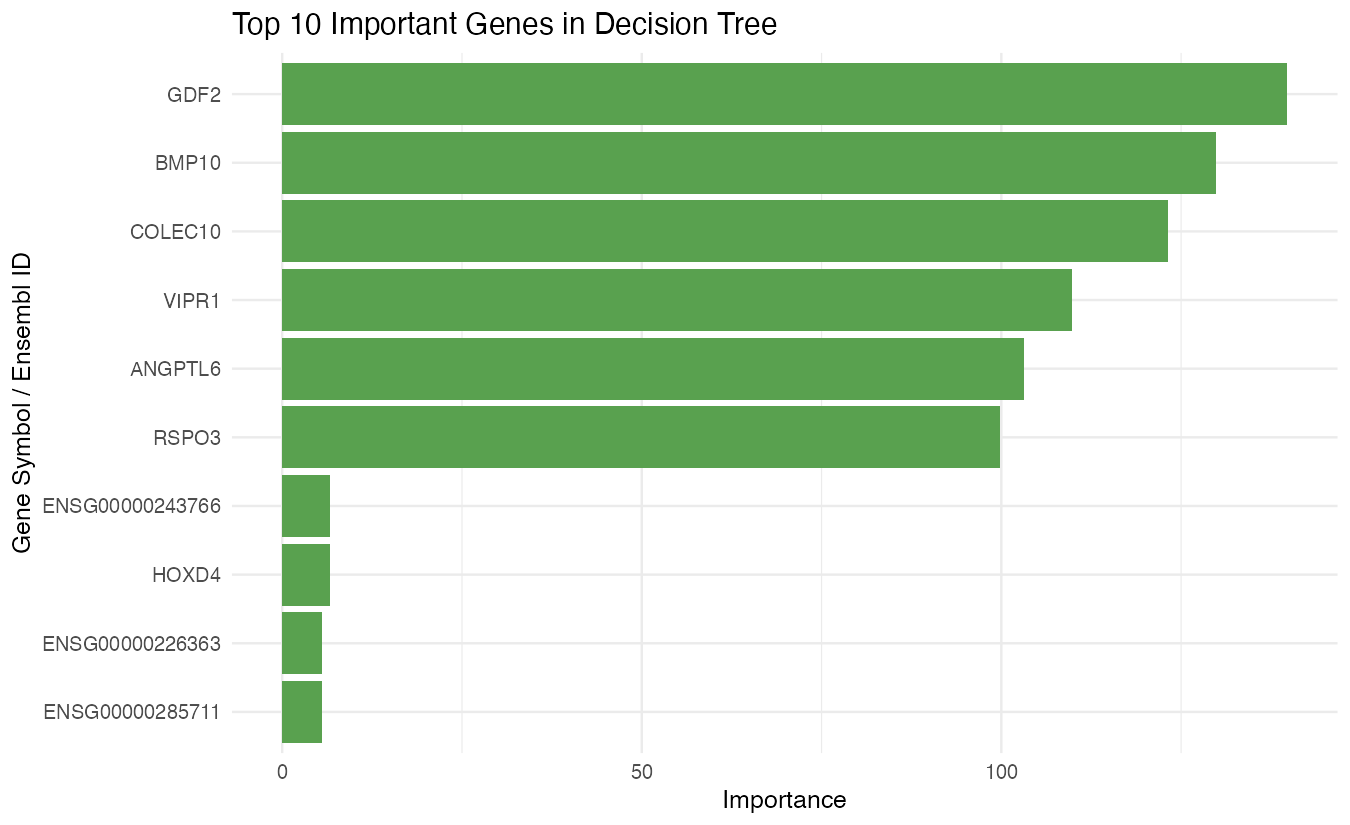
\includegraphics[width=0.72\textwidth]{tcga_hw_outputs/figures/decision_tree_variable_importance_top10.png}
\caption{决策树变量重要性前 10 基因}
\end{figure}

\begin{figure}[H]
\centering
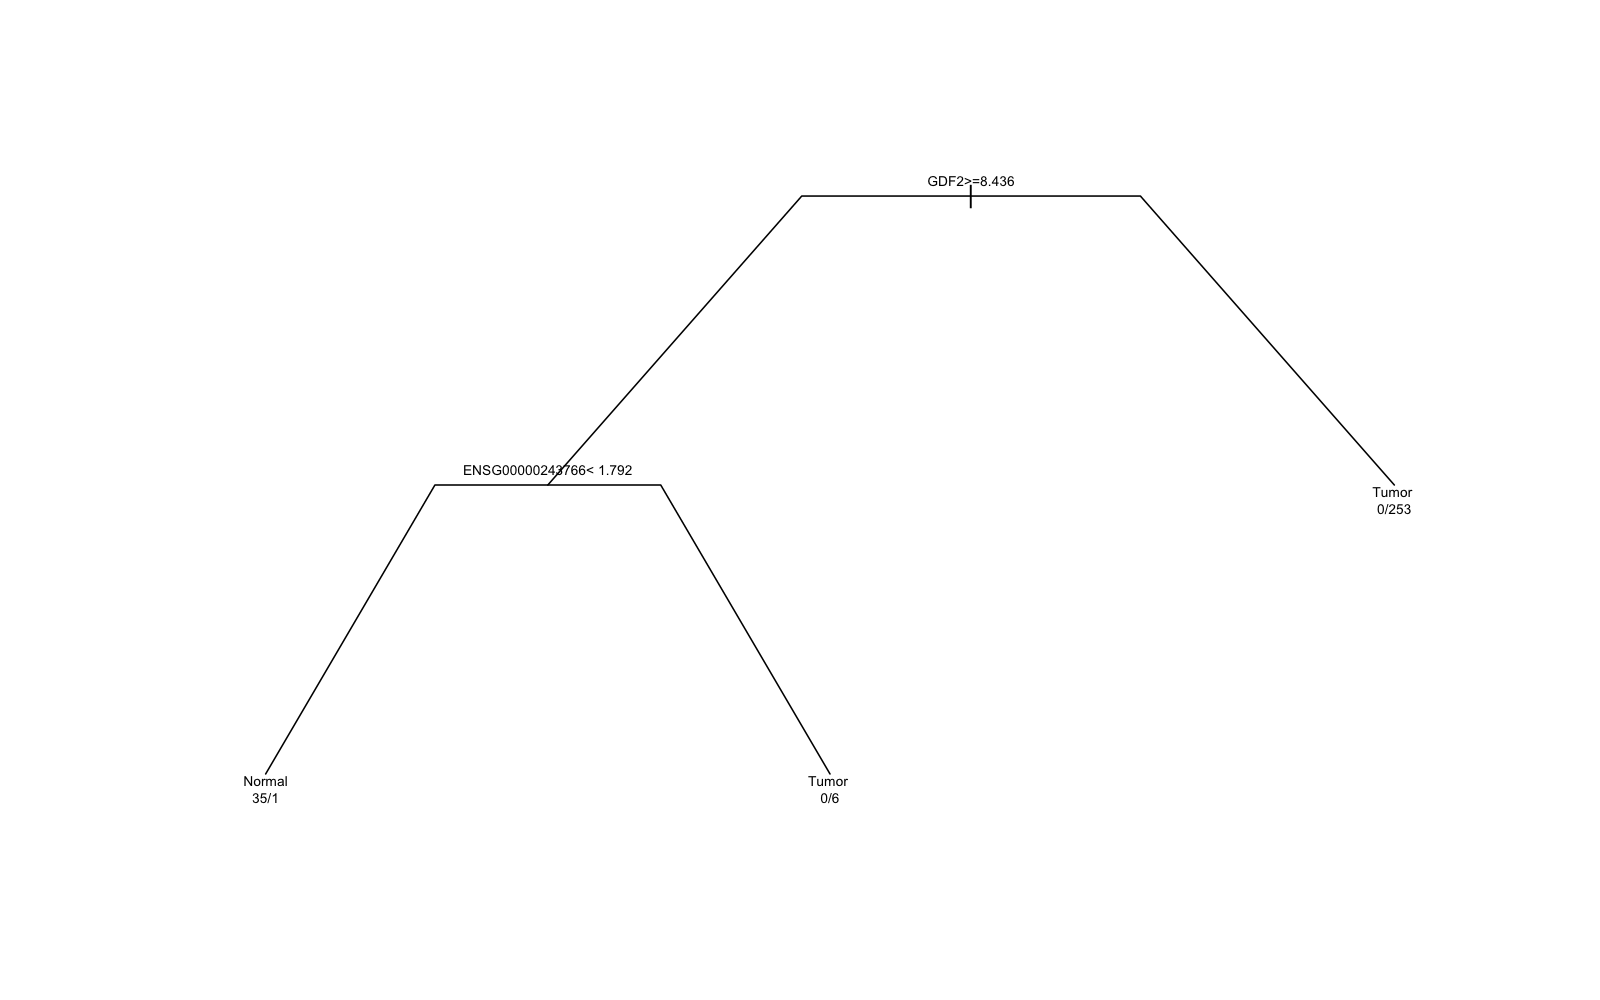
\includegraphics[width=\textwidth]{tcga_hw_outputs/figures/decision_tree_structure.png}
\caption{决策树结构图}
\end{figure}

根据变量重要性结果，排名靠前的基因包括 \texttt{GDF2}、\texttt{BMP10}、\texttt{FCN2}、\texttt{COLEC10} 和 \texttt{CLEC4M}。这些基因在决策树中被频繁用于分裂节点，说明它们对区分肿瘤与正常样本的贡献较大。

\section{讨论}
\subsection{为何选择这种方法}
这次选择决策树作为主要分类方法，主要有下面几个原因：
\begin{itemize}
  \item 决策树可直接处理多维表达特征，且不要求特征之间满足线性关系；
  \item 模型结构直观，便于解释哪些基因在分类中更重要；
  \item 对于本次样本量不大、特征数经筛选后为 50 的数据，决策树实现简单且适合课程实验要求。
\end{itemize}

\subsection{模型评价}
本实验是在独立测试集上做模型评价的。为了不只看一个准确率，这里还一起计算了 Precision、Recall、Specificity、F1 和 AUC。

这些指标分别反映了模型不同方面的表现：Accuracy 表示整体分对了多少；Precision 表示被判成肿瘤的样本里有多少是真的肿瘤；Recall 表示所有真实肿瘤里有多少被成功识别出来；Specificity 表示所有真实正常样本里有多少被正确分成正常；F1 是 Precision 和 Recall 的综合指标；AUC 则反映模型整体区分两类样本的能力。

\begin{table}[H]
\centering
\caption{决策树模型在测试集上的评价指标}
\begin{tabular}{cccccc}
\toprule
Accuracy & Precision & Recall & Specificity & F1 & AUC \\
\midrule
0.8730 & 0.9524 & 0.9009 & 0.6667 & 0.9259 & 0.7838 \\
\bottomrule
\end{tabular}
\end{table}

\begin{table}[H]
\centering
\caption{测试集混淆矩阵}
\begin{tabular}{ccc}
\toprule
实际类别 & 预测为 Normal & 预测为 Tumor \\
\midrule
Normal & 10 & 5 \\
Tumor & 11 & 100 \\
\bottomrule
\end{tabular}
\end{table}

从混淆矩阵可以看出，模型对肿瘤样本的识别效果比较好，肿瘤样本的召回率达到 0.9009；但对正常样本的识别相对弱一些，仍有 5 个正常样本被错分成肿瘤，所以 Specificity 只有 0.6667。出现这种情况的一个重要原因是原始数据里肿瘤样本远多于正常样本，模型更容易偏向肿瘤这一类。

\begin{figure}[H]
\centering
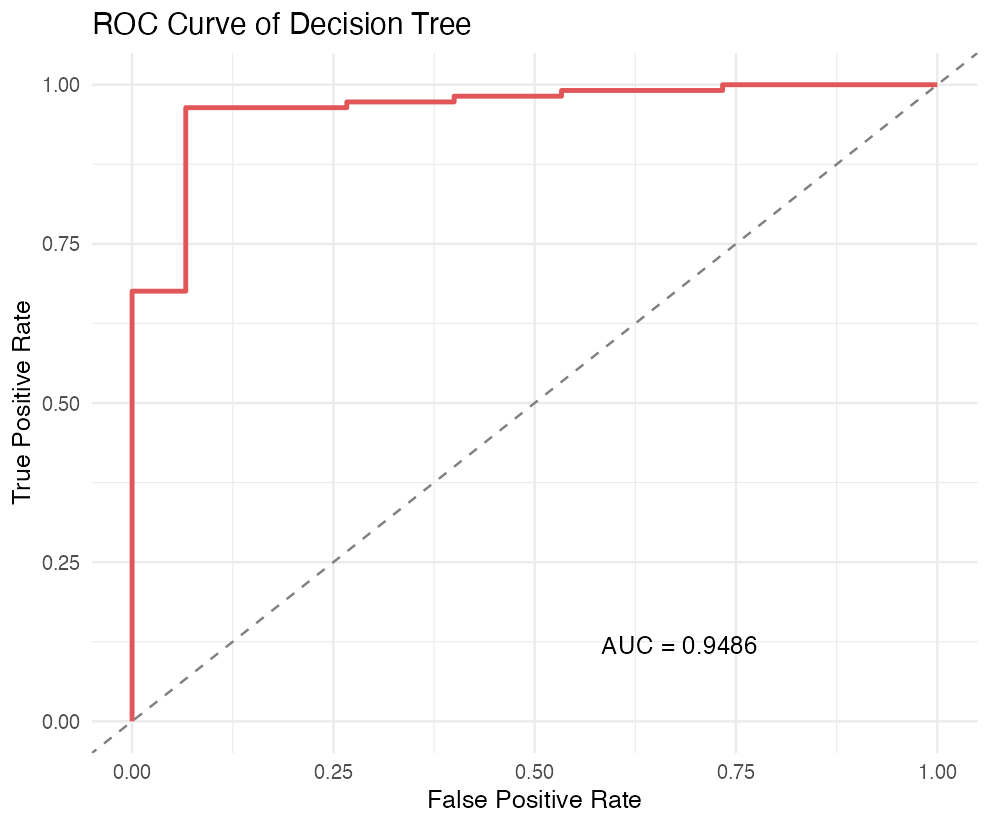
\includegraphics[width=0.62\textwidth]{tcga_hw_outputs/figures/roc_curve_decision_tree.png}
\caption{决策树模型 ROC 曲线}
\end{figure}

ROC 曲线对应的 AUC 为 0.7838，说明模型已经有一定的区分能力，明显好于随机猜测，但还谈不上特别理想，后面还有继续优化的空间。

\subsection{训练集选取基因的随机性及其影响}
这次实验是先随机划分训练集和测试集，再只在训练集里筛选 Top50 差异表达基因。因为训练集本身就是随机抽出来的，所以只要随机种子不同，进入训练集的样本组合就会变，最后筛出来的 Top50 基因也不一定完全一样。

这会带来两个比较直接的影响。第一，不同训练次数下得到的前 10 个差异基因和 Top50 特征集可能会有一些变化，尤其是排在边界附近的基因更容易被替换。第二，模型是基于这些特征训练出来的，所以不同训练次数下的分类结果也可能会波动，比如 Accuracy、AUC 或变量重要性排序都会有一些变化。

所以，这次实验得到的结果更适合理解为“在当前这一次随机划分下得到的可复现实验结果”，而不是一个完全固定不变的结论。如果想让结果更稳一些，后面可以考虑做重复随机划分、交叉验证，或者固定多个随机种子反复实验后再取平均。

\subsection{实验的不足与可改进方向}
这次实验还有几个比较明显的不足。首先，正常样本数明显少于肿瘤样本，类别不平衡会影响模型对正常样本的识别能力。其次，这里只做了一次训练集/测试集划分，所以结果会受到随机性的影响。再次，决策树虽然好解释，但泛化能力不一定比更强的集成方法更好。

后面如果继续做，可以尝试随机森林、支持向量机或者 XGBoost 这类方法，再结合交叉验证来得到更稳定的性能估计。另外，也可以把标准差异分析和机器学习里的特征筛选分得更清楚一些，这样结果解释会更自然。

\section{引用}
\subsection{数据集与软件}
\begin{itemize}
  \item 数据集：TCGA-LIHC 表达量数据，文件为 \texttt{TCGA-LIHC.star\_counts (2).tsv.gz}。
  \item 软件环境：R 4.5.2。
  \item 主要 R 包：\texttt{data.table} 1.17.8，\texttt{rpart} 4.1.24，\texttt{ggplot2} 4.0.0，\texttt{dplyr} 1.1.4，\texttt{tibble} 3.3.0，\texttt{clusterProfiler} 4.18.4，\texttt{org.Hs.eg.db} 3.22.0。
\end{itemize}

\subsection{AI 使用说明}
本实验在代码整理、报错排查、图表标签优化和实验报告撰写过程中使用了 AI 辅助。AI 主要帮助完成了以下工作：
\begin{itemize}
  \item 协助生成和修改 R 脚本，包括按样本类型区分肿瘤与正常样本、训练决策树模型，以及输出混淆矩阵、ROC 曲线和变量重要性图；
  \item 在代码运行过程中辅助分析报错原因并调整实现方式，例如基因 ID 转换、图像标签优化和 LaTeX 报告结构调整；
  \item 根据实验结果协助整理实验报告内容，使报告结构更符合实验报告范例要求。
\end{itemize}

需要说明的是，AI 主要作为辅助工具使用。所有代码均在本地环境中实际运行，所有结果、图表和表格均以本地运行输出为准；实验内容的组织、结果理解和最终表述经过了人工检查和修改。

\subsection{代表性提示词}
\begin{itemize}
  \item 仅基于训练集筛选 Top50 差异表达基因。
  \item 将 Ensembl ID 尽可能转换为基因名称，并在显著基因图和变量重要性图中优先显示基因名称。
  \item 套用更加规范的 LaTeX 模板。
\end{itemize}

\subsection{附：Vibe coding使用感受反思}

Vibe coding在本节课的使用中，无论是最开始的网站创建，还是在本实验代码生成和修改功能，都展现出了强大的能力。而在笔者的生活中，无论是实验数据处理、可视化，还是生活中其他需要的事情，Vibe coding均提供了非常方便也非常必要的帮助。
Vibe coding的出现使得没有编程基础的同学也可以轻松上手，在飞速发展的计算机时代利用更高效的工具达到自己的目的，这无疑是令人欣喜的。

然而，vibe coding的使用也并非是毫无技巧的工作。精准的提示词，对于遇到问题的精确描述，都是决定vibe coding过程效率和准确性的重要因素。
进一步而言，实现这些重要因素本身，需要使用者本人对于自己的工作目标，工作方法，工作方法基本原理，和期望达到的结果有清晰的认知。
对于生科院同学来说，一方面这证明着计算概论、数据结构与算法等基本课程的必要性，以及在使用相关方法与工具时对于其原理基本了解的重要性；
另一方面，也考验着我们将我们所需要的生物学知识融汇贯通，在vibe coding过程中紧扣根本生物学问题，而非为了“炫酷”的效果而提出画蛇添足的要求，实现华而不实的分析。

最后我想说，vibe coding的存在在表面上将“会编程”与“不会编程”的人之间的距离变得模糊。但不可否认的是，技术的进步始终是在给人类本身内化于心的知识、技能加码，他们或许会提高所有人的下限，同样也在不断拉大着利用技术所能达到的最高水平间的距离。
在AI等技术飞速发展的当下，即便是作为生科院的同学，也无时无刻不受着“自动化实验室”、“干实验取代湿实验”等言论的影响。仅仅以vibe coding的使用体验作为切口，我也将有信心于作为人本身的价值、有信息于学习的价值，更相信技术与人会形成健康和谐的关系，而非所谓的“你死我活”。

\end{document}
